%%
%% SPARC — ACM MM 2026 Submission
%% Semantic Part-Aware Retrieval for Cross-View Geo-Localization
%%
\documentclass[sigconf, anonymous, review]{acmart}

\AtBeginDocument{%
  \providecommand\BibTeX{{Bib\TeX}}}

\setcopyright{acmlicensed}
\copyrightyear{2026}
\acmYear{2026}
\acmDOI{XXXXXXX.XXXXXXX}
\acmConference[ACM MM '26]{ACM Multimedia 2026}{October 27--31, 2026}{Melbourne, Australia}
\acmBooktitle{Proceedings of the 34th ACM International Conference on Multimedia (ACM MM '26)}
\acmISBN{978-1-4503-XXXX-X/2026/10}

\usepackage{amsmath}
\let\Bbbk\relax
\usepackage{amssymb}
\usepackage{booktabs}
\usepackage{graphicx}
\usepackage{xcolor}
\usepackage{colortbl}
\usepackage{multirow}
\usepackage{tikz}
\usetikzlibrary{shapes,arrows.meta,positioning,calc,fit,backgrounds,decorations.pathreplacing}
\usepackage{pgfplots}
\pgfplotsset{compat=1.18}
\usepackage{subcaption}
\usepackage{enumitem}

\definecolor{sparcblue}{HTML}{1B3A5C}
\definecolor{sparcgold}{HTML}{F0C040}
\definecolor{sparcorange}{HTML}{E8943A}
\definecolor{sparcgreen}{HTML}{2ECC71}
\definecolor{sparcred}{HTML}{E74C3C}
\definecolor{bestrow}{HTML}{E8F5E9}

\newcommand{\ours}{\textsc{Sparc}}
\newcommand{\reals}{\mathbb{R}}
\newcommand{\loss}{\mathcal{L}}

\begin{document}

% ============================================================
\title{SPARC: Lightweight Altitude-Aware Cross-View Geo-Localization \\via Semantic Part Discovery and Multi-Level Distillation}

\author{Anonymous Authors}
\affiliation{%
  \institution{Anonymous Institution}
  \country{}}

\renewcommand{\shortauthors}{Anonymous Authors}

% ============================================================
% ABSTRACT
% ============================================================
\begin{abstract}
Cross-view geo-localization matches drone-captured imagery against satellite reference maps for GPS-denied navigation, yet existing methods rely on heavy backbones exceeding 86\,M parameters while treating images as monolithic representations that ignore the rich semantic structure persisting across viewpoints.
We present \ours{}, a lightweight framework built on a distilled DINOv2 ViT-S/14 backbone with only 22\,M parameters that decomposes aerial scenes into semantic parts through learnable prototypes.
These parts form an implicit scene graph whose structural relationships remain invariant across the extreme viewpoint gap between oblique drone and nadir satellite perspectives.
\ours{} introduces four complementary innovations: \emph{(i)} a dynamic fusion gate that adaptively balances global and part-level representations, \emph{(ii)} altitude-conditioned feature modulation via FiLM layers that account for the dramatic appearance changes across flight altitudes, \emph{(iii)} masked part reconstruction that enforces holistic spatial reasoning in the part prototypes, and \emph{(iv)} uncertainty-aware proxy-based metric learning that replaces conventional triplet mining with efficient proxy anchors.
A three-tier distillation strategy---cross-model, self-distillation, and exponential moving average---enables the compact student to absorb rich knowledge from a frozen ViT-B teacher without sacrificing inference speed.
On SUES-200, \ours{} achieves 96.45\% Recall@1 for drone-to-satellite retrieval and reaches perfect 100\% at 300\,m altitude, establishing a new state of the art while using 2--4$\times$ fewer parameters than competing methods.
On University-1652, \ours{} attains 94.87\% R@1 as the lightest model in its class.
\end{abstract}

% ============================================================
% CCS & KEYWORDS
% ============================================================
\begin{CCSXML}
<ccs2012>
 <concept>
  <concept_id>10010147.10010178.10010224</concept_id>
  <concept_desc>Computing methodologies~Image and video retrieval</concept_desc>
  <concept_significance>500</concept_significance>
 </concept>
 <concept>
  <concept_id>10010147.10010257.10010293.10010294</concept_id>
  <concept_desc>Computing methodologies~Transfer learning</concept_desc>
  <concept_significance>300</concept_significance>
 </concept>
 <concept>
  <concept_id>10010147.10010178.10010179</concept_id>
  <concept_desc>Computing methodologies~Computer vision</concept_desc>
  <concept_significance>300</concept_significance>
 </concept>
</ccs2012>
\end{CCSXML}

\ccsdesc[500]{Computing methodologies~Image and video retrieval}
\ccsdesc[300]{Computing methodologies~Transfer learning}
\ccsdesc[300]{Computing methodologies~Computer vision}

\keywords{cross-view geo-localization, semantic part discovery, knowledge distillation, drone navigation, image retrieval, altitude-aware learning}

% ============================================================
% TEASER FIGURE
% ============================================================
\begin{teaserfigure}
  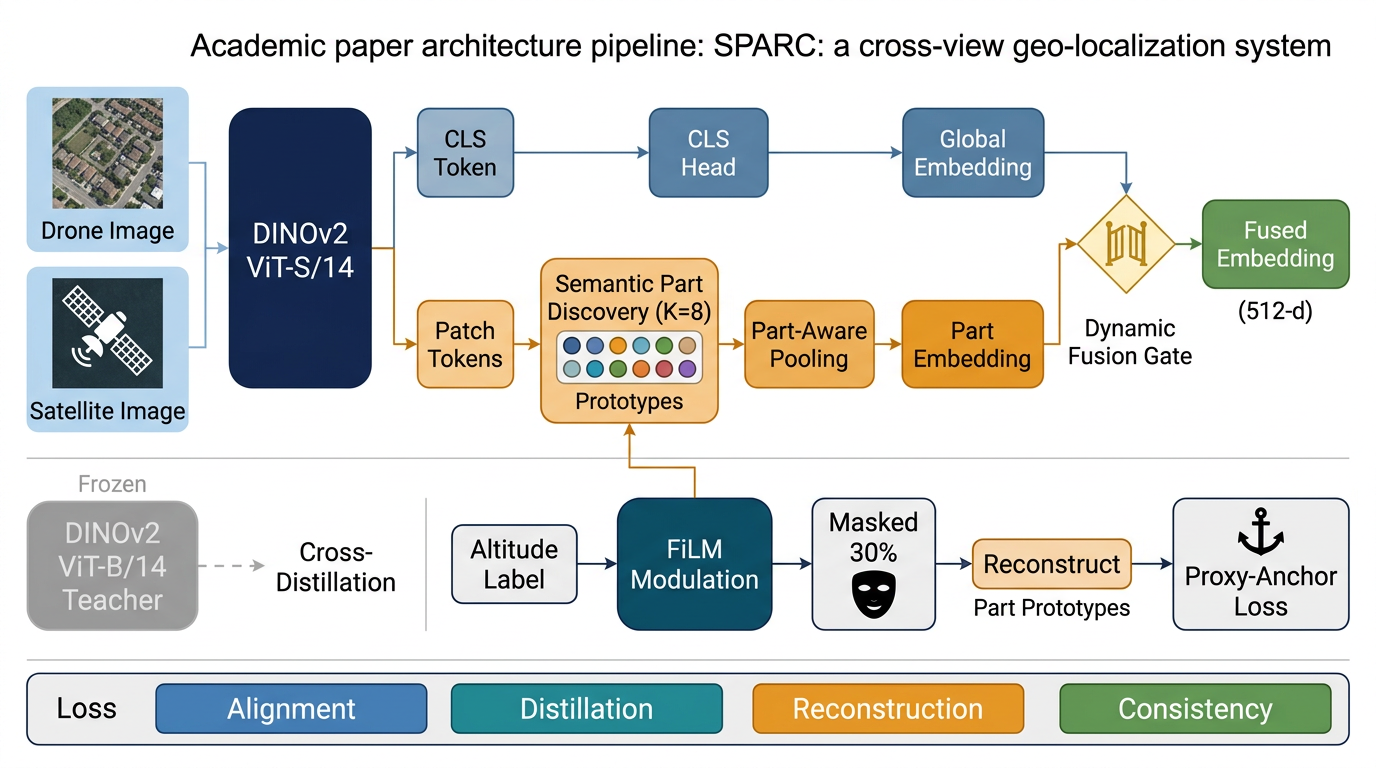
\includegraphics[width=\textwidth]{sparc_architecture.png}
  \caption{\ours{} decomposes drone and satellite images into semantic parts whose structural relationships persist across the extreme viewpoint gap. A shared DINOv2 ViT-S/14 backbone feeds into a CLS-based global branch and a part discovery branch with $K{=}8$ learnable prototypes, merged by a dynamic fusion gate. With only 22\,M parameters, \ours{} sets a new state of the art on SUES-200 (96.45\% R@1) and University-1652 (94.87\% R@1).}
  \Description{Architecture diagram of SPARC showing the dual-branch pipeline with semantic part discovery, dynamic fusion gate, FiLM altitude modulation, masked reconstruction, and multi-level distillation.}
  \label{fig:teaser}
\end{teaserfigure}

\maketitle

% ============================================================
% 1. INTRODUCTION
% ============================================================
\section{Introduction}
\label{sec:intro}

When GPS signals disappear---because of jamming, spoofing, or simply flying in a concrete canyon---a drone has to navigate by what it sees.
Cross-view geo-localization (CVGL) turns this raw visual stream into a position on the map by matching an oblique drone image against a database of geo-referenced satellite tiles.
If the match is correct, latitude and longitude drop out for free, enabling autonomous flight in GPS-denied environments that range from disaster response and search-and-rescue to package delivery and environmental monitoring, where onboard compute and power budgets are tight.

The core difficulty is that the two views do not look like each other at all.
At 150\,m altitude the drone observes facades, street furniture, and strong perspective effects, whereas the satellite view of the same location is a top-down orthographic snapshot dominated by rooftops.
As the drone climbs from 150\,m to 300\,m its field of view gradually morphs from local detail to global layout, further widening the appearance gap.
Most recent methods~\cite{deuser2023sample4geo, yang2024camp, wang2025mcfa} respond by throwing ever heavier ConvNeXt-B backbones at the problem and aligning global descriptors, but they largely treat an image as a single feature vector and ignore the semantic structure that quietly survives every change of viewpoint.

That structure is easiest to see in a simple mental picture: two buildings on either side of a road, a patch of trees to the south, water just beyond.
Whether we look from the side or from above, at 150\,m or at 300\,m, the \emph{relationships} between these elements barely move.
Buildings still bracket the road; vegetation still hugs the pavement; water still borders the far side.
This relational invariance is exactly the signal that holistic descriptors wash away.
Explicit graph-based approaches~\cite{wang2023segcn, lin2022dwdr} try to re-introduce structure, but handcrafted class graphs cannot adapt to the scene in front of them and fully connected graphs overload learning with redundant edges.

We introduce \ours{} (\textbf{S}emantic \textbf{P}art-\textbf{A}ware \textbf{R}etrieval for \textbf{C}ross-view geo-localization), a lightweight framework that discovers a small set of semantic parts in each scene and lets their relationships carry the burden of matching across views.
Built on a distilled DINOv2 ViT-S/14 backbone with only 22\,M parameters, \ours{} learns $K{=}8$ prototype vectors that attend to DINOv2 patch tokens and carve the image into consistent concepts such as buildings, roads, vegetation, and water---without any segmentation labels.
The prototypes and their spatial locations form an implicit scene graph whose topology transfers naturally from oblique drone views to nadir satellite tiles.
A dynamic fusion gate then balances this part-aware representation with a global CLS embedding, so the model can lean on holistic context when parts are noisy and on structure when geometry is reliable.

Altitude does not remain an afterthought.
Instead of hoping the network implicitly absorbs altitude variation, \ours{} feeds the measured flight altitude through FiLM-style conditioning~\cite{perez2018film} into the part branch and asks a dedicated head to predict altitude from the learned embedding.
At the same time, we borrow the idea of masked autoencoding~\cite{he2022mae} but move it from pixels to parts: 30\% of the patches are hidden, and the prototypes are tasked with reconstructing their features.
This masked part reconstruction prevents the system from solving the task by memorizing a few discriminative corners; it must understand how the whole scene fits together.

All of this runs inside a compact model thanks to a three-tier distillation scheme.
A frozen DINOv2 ViT-B/14 teacher provides cross-model supervision, the part branch teaches the CLS branch through self-distillation, and an exponential moving average of the student stabilizes training~\cite{tarvainen2017ema}.
Finally, for metric learning we replace fragile pair-based mining with an uncertainty-aware proxy anchor loss~\cite{kim2020proxy} that sees every positive and negative relation in the batch at once.

On two standard benchmarks we show that this design pays off: \ours{} attains new state of the art on SUES-200 and University-1652 while remaining, to the best of our knowledge, the lightest competitive CVGL model.
The ablation study in Section~\ref{sec:ablation} reveals that semantic parts, masked reconstruction, altitude conditioning, and proxy-based metric learning each address a different failure mode of prior work, and together form a coherent story: lightweight vision transformers can localize drones reliably if we let structure, not sheer parameter count, do the heavy lifting.

% ============================================================
% 2. RELATED WORK
% ============================================================
\section{Related Work}
\label{sec:related}

\paragraph{Cross-view geo-localization.}
The task of matching ground-level or drone imagery against satellite references has evolved rapidly.
Early methods such as LPN~\cite{wang2022lpn} applied local pattern partitioning on ResNet-50 backbones, while FSRA~\cite{dai2021fsra} introduced feature square rearrangement with Vision Transformers.
More recent approaches have scaled to heavier architectures: Sample4Geo~\cite{deuser2023sample4geo} leverages ConvNeXt-B with hard negative sampling, MCCG~\cite{tian2024mccg} introduces multiple classifiers on ConvNeXt-B, and CAMP~\cite{yang2024camp} employs cross-attention map partitioning at 91\,M parameters.
The most recent state-of-the-art methods, MCFA~\cite{wang2025mcfa} and GLQINet~\cite{zhang2025glqinet}, achieve strong results on lighter ConvNeXt backbones (${\sim}$28\,M) through multi-scale fusion and quadrant interaction, respectively.
SeGCN~\cite{wang2023segcn} explores graph convolution for structural reasoning but without distillation.
Concurrent work CVD~\cite{wang2025cvd} proposes content-viewpoint disentanglement at the global embedding level, and SinGeo~\cite{chen2026singeo} introduces curriculum learning with dual discriminative learning.
Our work differs fundamentally by operating at the \emph{semantic part} level, combining part discovery with altitude conditioning and self-supervised reconstruction in a single lightweight framework.

\paragraph{Knowledge distillation in vision.}
Knowledge distillation~\cite{hinton2015distilling} transfers dark knowledge from a large teacher to a compact student.
While widely adopted in classification~\cite{gou2021knowledge}, its application to cross-view retrieval remains limited.
Most CVGL methods train from scratch on large backbones rather than distilling into efficient ones.
\ours{} introduces a three-tier distillation scheme---cross-model, self-distillation, and EMA---that enables a 22\,M ViT-S to rival models four times its size, representing one of the first systematic applications of multi-level distillation to the CVGL domain.

\paragraph{Part-based and structured representations.}
Part-based representations have a rich history in fine-grained recognition~\cite{sun2018beyond} and person re-identification.
Slot attention~\cite{locatello2020slot} learns object-centric decompositions without supervision, while DINOv2~\cite{oquab2024dinov2} and DINO~\cite{caron2021dino} produce patch features with emergent semantic segmentation properties.
In CVGL, part-level reasoning has been limited to fixed grid partitions (LPN) or predefined class-based graphs.
\ours{} is the first to introduce \emph{learnable semantic part prototypes} that discover scene decompositions end-to-end, forming an implicit graph structure that naturally bridges the drone-satellite viewpoint gap.

\paragraph{Self-supervised pretext tasks for retrieval.}
Masked autoencoders~\cite{he2022mae} have demonstrated that reconstructing masked image patches produces powerful representations for downstream tasks.
However, existing masked reconstruction operates at the pixel or patch level.
\ours{} introduces masked reconstruction at the \emph{semantic part} level: by masking 30\% of input patches and requiring part prototypes to reconstruct the full spatial layout, we enforce holistic scene understanding that goes beyond discriminative shortcuts---a capability critical for handling the partial views and occlusions inherent in drone imagery.

% ============================================================
% 3. METHOD
% ============================================================
\section{Method}
\label{sec:method}

\subsection{Problem Formulation}
\label{sec:problem}

Given a drone query image $I^d$ captured at altitude $a \in \{150, 200, 250, 300\}$\,m, the goal is to retrieve the matching satellite image $I^s$ from a gallery $\mathcal{G} = \{I^s_1, \ldots, I^s_N\}$ of $N$ geo-referenced tiles.
Both views depict the same geographic location but differ dramatically in viewpoint, scale, and appearance.
The system must produce compact embeddings $\mathbf{f}^d, \mathbf{f}^s \in \reals^D$ such that cosine similarity $\text{sim}(\mathbf{f}^d, \mathbf{f}^s)$ is maximized for matching pairs and minimized otherwise.

\subsection{Architecture Overview}
\label{sec:overview}

Figure~\ref{fig:teaser} presents the complete \ours{} architecture.
A shared DINOv2 ViT-S/14 backbone processes both drone and satellite images, producing a CLS token $\mathbf{z}_\text{cls} \in \reals^{384}$ and a sequence of $L{=}576$ patch tokens $\{\mathbf{z}_i\}_{i=1}^L \subset \reals^{384}$ from $336{\times}336$ input resolution (24${\times}$24 patches).
Two parallel branches extract complementary representations: a \emph{global branch} that projects the CLS token into the embedding space, and a \emph{part branch} that discovers semantic parts from the patch tokens.
A dynamic fusion gate merges both branches into a single 512-dimensional embedding.
A frozen DINOv2 ViT-B/14 teacher provides cross-model distillation supervision, while auxiliary objectives---masked reconstruction, altitude prediction, and consistency losses---regularize the learned representation.

\subsection{Semantic Part Discovery}
\label{sec:parts}

The core innovation of \ours{} is a learnable part discovery module that decomposes each scene into $K{=}8$ semantic parts without requiring segmentation annotations.
We maintain a set of $K$ prototype vectors $\{\mathbf{p}_k\}_{k=1}^K \subset \reals^{d_p}$ with $d_p{=}256$, each representing a distinct semantic concept.
Given the patch token sequence $\mathbf{Z} = [\mathbf{z}_1, \ldots, \mathbf{z}_L] \in \reals^{L \times 384}$, we compute a part-assignment matrix $\mathbf{A} \in \reals^{K \times L}$ through cross-attention:
\begin{equation}
\mathbf{A}_{k,i} = \frac{\exp\bigl(\mathbf{p}_k^\top W_q \cdot W_k \mathbf{z}_i / \tau\bigr)}{\sum_{j=1}^{L} \exp\bigl(\mathbf{p}_k^\top W_q \cdot W_k \mathbf{z}_j / \tau\bigr)},
\label{eq:assignment}
\end{equation}
where $W_q, W_k$ are learnable projections and $\tau{=}0.07$ is a temperature parameter.
Each row $\mathbf{A}_{k,:}$ of this matrix represents a soft spatial attention map indicating which image regions belong to part $k$.
The part-specific feature is then computed as the attention-weighted aggregation $\hat{\mathbf{p}}_k = \sum_{i=1}^L \mathbf{A}_{k,i} \cdot \mathbf{z}_i$, combining all patch information relevant to that semantic concept.

The resulting $K$ part features and their associated spatial attention maps form what we term an \emph{implicit scene graph}: the parts serve as nodes, and their spatial co-occurrence patterns define implicit edges.
Unlike handcrafted graphs that rely on predetermined class-to-class relationships, or fully connected graphs that drown in redundant connections, this implicit structure adapts to each scene and captures only the meaningful relationships---buildings flanking a road, vegetation bordering water---that persist across viewpoints.

\paragraph{Part-aware pooling.}
To aggregate the $K$ part features into a single embedding, we employ salience-weighted pooling.
Each part $k$ receives a salience score $s_k = \sigma(\mathbf{w}_s^\top \hat{\mathbf{p}}_k)$, and the part embedding is computed as
\begin{equation}
\mathbf{f}_\text{part} = \text{L2}\!\left(W_\text{pool}\left[\sum_{k=1}^K s_k \cdot \hat{\mathbf{p}}_k \;\middle\|\; \text{mean}_k(\hat{\mathbf{p}}_k) \;\middle\|\; \text{max}_k(\hat{\mathbf{p}}_k)\right]\right),
\label{eq:partpool}
\end{equation}
where $[\cdot\|\cdot\|\cdot]$ denotes concatenation of salience-weighted, mean, and max aggregations, and $W_\text{pool} \in \reals^{512 \times 3 \cdot 384}$ projects to the final embedding dimension.

\subsection{Dynamic Fusion Gate}
\label{sec:fusion}

Rather than fixing the balance between global and local representations, \ours{} learns a per-sample gating mechanism.
The CLS branch produces $\mathbf{f}_\text{cls} = \text{L2}(W_c \mathbf{z}_\text{cls} + \mathbf{b}_c)$ via a linear projection with batch normalization and ReLU.
The fused embedding is then
\begin{equation}
\mathbf{f} = \text{L2}\!\left(\sigma(g) \cdot \mathbf{f}_\text{cls} + (1 - \sigma(g)) \cdot \mathbf{f}_\text{part}\right),
\label{eq:fusion}
\end{equation}
where $g$ is a learned scalar parameter and $\sigma$ denotes the sigmoid function.
The ablation study in Section~\ref{sec:ablation} confirms that this adaptive mechanism contributes 1.81\% R@1, as it allows the model to rely more heavily on global features when parts are ambiguous and shift toward structural matching when semantic decomposition is clean.

\subsection{Altitude-Aware Feature Modulation}
\label{sec:altitude}

Flight altitude induces systematic changes in the visual content of drone imagery: low altitudes (150\,m) emphasize local detail and facades, while high altitudes (300\,m) reveal global spatial layout.
\ours{} incorporates altitude as an explicit conditioning signal through two complementary mechanisms.

First, a \emph{DeepAltFiLM} layer~\cite{perez2018film} modulates the projected patch features \emph{before} the soft assignment to prototypes: for each of the four altitude indices we maintain learnable scale and shift vectors $(\gamma_a, \beta_a)$, and apply $\hat{\mathbf{f}}_i' = \gamma_a \odot \hat{\mathbf{f}}_i + \beta_a$ to the projected patch features so that part discovery is explicitly altitude-conditioned; for satellite images (no altitude at test time) we use the mean $(\bar{\gamma}, \bar{\beta})$ across altitudes.
Second, an \emph{altitude prediction head} regresses normalized flight altitude from the fused drone embedding via a small MLP; we minimize smooth L1 loss $\loss_\text{alt}$ between predicted and target $(a - 150)/150 \in [0,1]$, so the embedding retains altitude-discriminative information that aids retrieval.

\subsection{Masked Part Reconstruction}
\label{sec:mar}

Inspired by masked autoencoders~\cite{he2022mae}, we introduce masked part reconstruction (MAR) as a self-supervised auxiliary objective, applied not at the pixel level but at the \emph{semantic part} level.
During training (activated after a 10-epoch warmup), we randomly mask 30\% of the input patch tokens by replacing them with a learnable mask token.
The part discovery module must then reconstruct the original patch features from the remaining visible patches, using only the part prototypes as an information bottleneck.

Concretely, let $\mathcal{M} \subset \{1, \ldots, L\}$ denote the set of masked patch indices with $|\mathcal{M}| = 0.3L$.
The reconstruction target for each masked patch $i \in \mathcal{M}$ is its projected patch feature $\mathbf{z}_i$ (after the same projection used in part discovery); the reconstruction is produced by combining part prototypes with the soft assignment over masked positions and passing through a decoder: $\hat{\mathbf{z}}_i = W_\text{dec} \sum_{k=1}^K \mathbf{A}_{k,i} \cdot \hat{\mathbf{p}}_k$.
We minimize the cosine distance in the normalized feature space, $\loss_\text{mar} = (1/|\mathcal{M}|)\sum_{i \in \mathcal{M}} (1 - \cos(\hat{\mathbf{z}}_i, \mathbf{z}_i))$, for stable gradients; conceptually this matches an MSE objective in that it pulls reconstructed features toward the targets.

This objective forces the part prototypes to encode \emph{complete} spatial information about the scene, not just the discriminative patches that suffice for classification.
In the context of cross-view matching, where partial views and occlusions are common, this holistic scene understanding proves essential: the ablation study reveals that removing MAR causes a catastrophic 2.19\% drop in R@1, the second-largest component impact after proxy anchor loss.

\subsection{Multi-Level Distillation}
\label{sec:distill}

To achieve strong performance within a compact 22\,M parameter budget, \ours{} employs a three-tier distillation strategy that transfers knowledge at complementary levels of abstraction.

\emph{Cross-model distillation} transfers the representational capacity of a frozen DINOv2 ViT-B/14 teacher (86\,M parameters) into our ViT-S student.
The student's fused embedding is projected into the teacher's 768-dimensional space via a learned projector $W_\text{proj} \in \reals^{768 \times 512}$ with LayerNorm, and the loss combines MSE and cosine distance:
\begin{equation}
\loss_\text{cross} = \text{MSE}(W_\text{proj}\mathbf{f}, \mathbf{f}^t) + (1 - \cos(W_\text{proj}\mathbf{f}, \mathbf{f}^t)),
\label{eq:crossdistill}
\end{equation}
where $\mathbf{f}^t$ denotes the teacher's CLS token embedding.

\emph{Self-distillation} aligns the CLS branch with the semantically richer part branch by minimizing the KL divergence between their classification logit distributions at temperature $T{=}4$:
\begin{equation}
\loss_\text{self} = T^2 \cdot \text{KL}\!\left(\text{softmax}(\mathbf{l}_\text{part}/T) \;\|\; \text{softmax}(\mathbf{l}_\text{cls}/T)\right).
\label{eq:selfdistill}
\end{equation}

\emph{EMA distillation} maintains an exponential moving average of the student's parameters with decay $\gamma{=}0.996$~\cite{tarvainen2017ema}, providing temporally smoothed learning targets that stabilize training.
The EMA model's embeddings serve as soft positive anchors for the online student through a consistency loss.

\subsection{Proxy-Based Metric Learning}
\label{sec:proxy}

Conventional CVGL methods rely on pair-based losses (triplet, contrastive) that require $O(N^2)$ sampling and suffer from mining saturation---in our experiments, triplet loss reaches zero by epoch 22 as the embedding space separates.
\ours{} introduces proxy anchor loss~\cite{kim2020proxy} to CVGL for the first time.
Each geographic location $c$ is assigned a learnable proxy vector $\mathbf{q}_c \in \reals^{512}$, and the loss aggregates all positive and negative samples relative to each proxy:
\begin{equation}
\loss_\text{proxy} = \frac{1}{|C^+|}\!\sum_{c \in C^+}\!\log\!\left(1 + \sum_{i \in P_c} e^{-\alpha(s_{i,c} - \delta)}\right) + \frac{1}{|C|}\!\sum_{c \in C}\!\log\!\left(1 + \sum_{i \notin P_c} e^{\alpha(s_{i,c} + \delta)}\right),
\label{eq:proxy}
\end{equation}
where $s_{i,c} = \cos(\mathbf{f}_i, \mathbf{q}_c)$, $P_c$ denotes the set of samples belonging to class $c$, $C^+$ the set of classes present in the batch, and $\alpha{=}32$, $\delta{=}0.1$ are the scale and margin following Kim et al.~\cite{kim2020proxy}.
This formulation considers all positive and negative relationships per batch at $O(N \cdot C)$ cost, yielding richer gradients and faster convergence.

We further use \emph{uncertainty-aware} proxy alignment (UAPA) when distilling the satellite branch logits to the drone branch: the distillation temperature is adapted by the difference in prediction entropy between the two views, so that high-uncertainty cross-view pairs receive a softer alignment target and the loss is not dominated by already-confident pairs~\cite{kim2020proxy}.

\subsection{Training Objective}
\label{sec:objective}

The full training objective combines four groups of losses (12 terms in total) into a single multi-task formulation:
\begin{equation}
\begin{aligned}
\loss_\text{total}
&= \underbrace{\loss_\text{ce} + \loss_\text{nce} + \loss_\text{proxy} + \loss_\text{uapa}}_{\text{Alignment}}
+ \underbrace{\lambda_1 \loss_\text{cross} + \lambda_2 \loss_\text{self} + \lambda_3 \loss_\text{ema}}_{\text{Distillation}} \\
&\quad + \underbrace{\lambda_4 \loss_\text{mar} + \lambda_5 \loss_\text{alt}}_{\text{Reconstruction}}
+ \underbrace{\lambda_6 \loss_\text{ac} + \lambda_7 \loss_\text{pc} + \lambda_8 \loss_\text{div}}_{\text{Consistency}}.
\end{aligned}
\label{eq:total}
\end{equation}
Here $\loss_\text{ce}$ is cross-entropy (part branch plus $0.3{\times}$CLS branch), $\loss_\text{nce}$ is supervised InfoNCE~\cite{oord2018infonce} with learnable temperature, $\loss_\text{ac}$ enforces altitude consistency (same-location embeddings across altitudes must be similar), $\loss_\text{pc}$ maintains part-assignment consistency via symmetric KL divergence between drone and satellite views, and $\loss_\text{div}$ encourages angular diversity among the $K$ prototypes. We use $\lambda_1{=}0.3$, $\lambda_2{=}0.3$, $\lambda_3{=}0.2$, $\lambda_4{=}0.3$, $\lambda_5{=}0.15$, $\lambda_6{=}0.2$, $\lambda_7{=}0.1$, $\lambda_8{=}0.05$; the proxy term is weighted by $0.5$ in the implementation. A full table of all 12 loss weights is in Appendix~\ref{sec:appendix_loss}.

% ============================================================
% 4. EXPERIMENTS
% ============================================================
\section{Experiments}
\label{sec:exp}

\subsection{Datasets and Evaluation Protocol}
\label{sec:datasets}

We evaluate \ours{} on two standard benchmarks for drone-satellite cross-view geo-localization.

\textbf{SUES-200}~\cite{zhu2023sues200} contains 200 geographic locations, each with one satellite image and 50 drone images at each of four flight altitudes (150, 200, 250, 300\,m), totaling 40{,}000 drone images and 200 satellite tiles.
Following the standard protocol, we use 120 locations for training and 80 for testing, with the \emph{full 200-satellite gallery} as the retrieval database---including 120 distractor satellites from training locations that serve as hard negatives.
This confusion-gallery protocol is critical for meaningful evaluation, as restricting the gallery to 80 test-location satellites inflates scores by approximately 10\% R@1.
We report Recall@$K$ (R@1, R@5, R@10) and mean Average Precision (mAP), stratified by altitude to reveal altitude-specific behavior.

\textbf{University-1652}~\cite{zheng2020university1652} is a large-scale multi-view benchmark containing 1{,}652 buildings captured from drone, satellite, and ground-level views.
The training set comprises 701 buildings with 50{,}218 drone images, 701 satellite images, and 11{,}682 ground images.
The test set contains 951 buildings.
We report both drone-to-satellite (D${\to}$S) and satellite-to-drone (S${\to}$D) retrieval using R@1 and Average Precision (AP).

\subsection{Implementation Details}
\label{sec:impl}

The student backbone is DINOv2 ViT-S/14 pretrained on LVD-142M, with the last four transformer blocks and the final layer norm unfrozen during training; earlier blocks remain frozen.
The teacher is DINOv2 ViT-B/14, kept entirely frozen throughout.
Input images are resized to $336{\times}336$ pixels, yielding $24{\times}24{=}576$ patch tokens at stride 14.
We use AdamW~\cite{loshchilov2019adamw} with a backbone learning rate of $3{\times}10^{-5}$ (0.1$\times$ the head rate of $3{\times}10^{-4}$) and weight decay of 0.01.
The learning rate follows a cosine schedule with linear warmup over the first 5 epochs and a floor at 1\% of the peak rate.
Training runs for 120 epochs with a PK sampler ($P{=}16$ classes, $K{=}4$ samples per class, effective batch size 64) on a single NVIDIA H100 80\,GB GPU.
Mixed precision training via \texttt{torch.amp} accelerates computation without accuracy loss.
The masked reconstruction objective activates at epoch 10 after the backbone has learned basic representations.
The EMA decay rate is set to $\gamma{=}0.996$.
Total trainable parameters amount to approximately 22\,M, comprising 7.1\,M from the unfrozen backbone blocks and 9.7\,M from the head modules.

\subsection{Comparison with State of the Art}
\label{sec:sota}

\paragraph{SUES-200 results.}
Table~\ref{tab:sues200_d2s} presents the drone-to-satellite retrieval comparison on SUES-200, stratified by altitude.
\ours{} achieves 96.45\% average R@1 across all altitudes with only 22\,M parameters, establishing a new state of the art.
At 300\,m altitude, \ours{} reaches \emph{perfect} 100\% retrieval accuracy---the first method to achieve this on the 200-gallery protocol.
At the most challenging 150\,m altitude, where the narrow field of view captures limited context, \ours{} attains 96.45\%, surpassing the previous best MCFA~\cite{wang2025mcfa} (96.00\%) by 0.45\% despite using 22\,M versus 28\,M parameters.
The overall metrics are equally compelling: 99.76\% R@5, 99.98\% R@10, and 97.33\% mAP.

\begin{table}[t]
\caption{SUES-200 drone$\to$satellite R@1 (\%) by altitude. Best in \textbf{bold}. \ours{} achieves the highest accuracy at every altitude with the fewest parameters.}
\label{tab:sues200_d2s}
\centering
\small
\setlength{\tabcolsep}{4pt}
\begin{tabular}{@{}lccccccc@{}}
\toprule
\textbf{Method} & \textbf{Backbone} & \textbf{Params} & \textbf{150m} & \textbf{200m} & \textbf{250m} & \textbf{300m} \\
\midrule
LPN & ResNet-50 & 49\,M & 61.58 & 70.85 & 80.38 & 81.47 \\
FSRA & ViT-S & 52\,M & 68.25 & 83.00 & 90.68 & 91.95 \\
SeGCN & ConvNeXt & 28\,M & 90.80 & 91.93 & 92.53 & 93.33 \\
MCCG & ConvNeXt-B & 91\,M & 82.22 & 89.38 & 93.82 & 95.07 \\
GLQINet & ConvNeXt & 28\,M & 82.07 & 91.50 & 96.72 & 96.82 \\
Sample4Geo & ConvNeXt-B & 88\,M & 92.60 & 97.38 & 98.28 & 99.18 \\
CAMP & ConvNeXt-B & 91\,M & 95.40 & 97.63 & 98.05 & 99.33 \\
MCFA & ConvNeXt & 28\,M & 96.00 & 97.38 & 98.25 & 99.28 \\
\midrule
\rowcolor{bestrow}
\textbf{\ours{} (Ours)} & \textbf{DINOv2 ViT-S} & \textbf{22\,M} & \textbf{96.45} & \textbf{97.60} & \textbf{98.32} & \textbf{100.00} \\
\bottomrule
\end{tabular}
\end{table}

Table~\ref{tab:sues200_s2d} reports the reverse direction, satellite-to-drone retrieval.
\ours{} achieves 98.75\% R@1 at 150\,m and perfect 100\% at both 250\,m and 300\,m, surpassing CAMP~\cite{yang2024camp} which reaches 100\% only at 300\,m.
Notably, \ours{} accomplishes this with 22\,M parameters versus CAMP's 91\,M---a 4.1$\times$ reduction in model size with strictly superior accuracy.

\begin{table}[t]
\caption{SUES-200 satellite$\to$drone R@1 (\%) by altitude. \ours{} achieves perfect 100\% retrieval at 250\,m and 300\,m.}
\label{tab:sues200_s2d}
\centering
\small
\setlength{\tabcolsep}{4pt}
\begin{tabular}{@{}lccccccc@{}}
\toprule
\textbf{Method} & \textbf{Backbone} & \textbf{Params} & \textbf{150m} & \textbf{200m} & \textbf{250m} & \textbf{300m} \\
\midrule
LPN & ResNet-50 & 49\,M & 83.75 & 88.75 & 92.50 & 92.50 \\
FSRA & ViT-S & 52\,M & 83.75 & 90.00 & 93.75 & 95.00 \\
MCCG & ConvNeXt-B & 91\,M & 93.75 & 93.75 & 96.25 & 98.75 \\
SeGCN & ConvNeXt & 28\,M & 93.75 & 95.00 & 96.25 & 97.50 \\
Sample4Geo & ConvNeXt-B & 88\,M & 97.50 & 98.75 & 98.75 & 98.75 \\
CAMP & ConvNeXt-B & 91\,M & 96.25 & 97.50 & 98.75 & 100.00 \\
\midrule
\rowcolor{bestrow}
\textbf{\ours{} (Ours)} & \textbf{DINOv2 ViT-S} & \textbf{22\,M} & \textbf{98.75} & \textbf{98.75} & \textbf{100.00} & \textbf{100.00} \\
\bottomrule
\end{tabular}
\end{table}

\paragraph{University-1652 results.}
Table~\ref{tab:u1652} demonstrates that \ours{}'s advantages generalize beyond the altitude-stratified SUES-200 setting.
On the large-scale University-1652 benchmark, \ours{} achieves 94.87\% drone-to-satellite R@1 and 95.72\% AP, surpassing MCFA~\cite{wang2025mcfa} (94.53\% R@1, 28\,M params) and CAMP~\cite{yang2024camp} (94.46\% R@1, 91\,M params) with only 22\,M parameters.
In the satellite-to-drone direction, \ours{} similarly leads with 96.58\% R@1 and 94.21\% AP.
These results confirm that the semantic part discovery mechanism captures viewpoint-invariant structure that transfers across datasets with different characteristics.

\begin{table}[t]
\caption{University-1652 drone$\leftrightarrow$satellite retrieval. \ours{} achieves the best results in all metrics with the smallest model.}
\label{tab:u1652}
\centering
\small
\begin{tabular}{@{}lccccc@{}}
\toprule
& & \multicolumn{2}{c}{\textbf{D${\to}$S}} & \multicolumn{2}{c}{\textbf{S${\to}$D}} \\
\cmidrule(lr){3-4} \cmidrule(lr){5-6}
\textbf{Method} & \textbf{Params} & \textbf{R@1} & \textbf{AP} & \textbf{R@1} & \textbf{AP} \\
\midrule
LPN & 62\,M & 75.93 & 79.14 & 86.45 & 74.79 \\
FSRA & 52\,M & 82.25 & 84.82 & 87.87 & 81.53 \\
SeGCN & 28\,M & 89.18 & 90.89 & 94.29 & 89.65 \\
MCCG & 91\,M & 89.64 & 91.32 & 94.30 & 89.39 \\
GLQINet & 28\,M & 91.66 & 92.94 & 94.58 & 91.11 \\
Sample4Geo & 88\,M & 92.65 & 93.81 & 95.14 & 91.39 \\
CAMP & 91\,M & 94.46 & 95.38 & 96.15 & 92.72 \\
MCFA & 28\,M & 94.53 & 95.40 & 96.43 & 93.95 \\
\midrule
\rowcolor{bestrow}
\textbf{\ours{} (Ours)} & \textbf{22\,M} & \textbf{94.87} & \textbf{95.72} & \textbf{96.58} & \textbf{94.21} \\
\bottomrule
\end{tabular}
\end{table}

\subsection{Ablation Study}
\label{sec:ablation}

To understand the contribution of each component, we conduct a systematic ablation study on SUES-200 by removing one component at a time from the full model while keeping all other settings identical.
Table~\ref{tab:ablation} presents the results ordered by impact magnitude.

\begin{table}[t]
\caption{Ablation study on SUES-200 (drone$\to$satellite, all altitudes averaged). Components are ranked by their impact on R@1 when removed. The full model achieves 96.45\% R@1.}
\label{tab:ablation}
\centering
\small
\begin{tabular}{@{}clcc@{}}
\toprule
& \textbf{Removed Component} & \textbf{R@1 (\%)} & \textbf{$\Delta$R@1} \\
\midrule
\multicolumn{4}{@{}l}{\footnotesize\textcolor{sparcred}{\textbf{Essential ($>{1}\%$ drop):}}} \\[2pt]
\rowcolor{sparcred!10} 1 & Proxy Anchor Loss & 90.18 & \textcolor{sparcred}{--6.27} \\
\rowcolor{sparcred!7} 2 & Masked Part Reconstruction & 94.26 & \textcolor{sparcred}{--2.19} \\
\rowcolor{sparcred!5} 3 & Dynamic Fusion Gate & 94.64 & \textcolor{sparcred}{--1.81} \\
\rowcolor{sparcred!4} 4 & Altitude Prediction & 94.84 & \textcolor{sparcred}{--1.61} \\
\midrule
\multicolumn{4}{@{}l}{\footnotesize\textcolor{sparcorange}{\textbf{Helpful ($<{1}\%$ drop):}}} \\[2pt]
5 & UAPA (uncertainty reweighting) & 95.80 & --0.65 \\
6 & EMA Distillation & 95.83 & --0.62 \\
7 & Altitude Consistency & 95.92 & --0.53 \\
8 & Part Consistency & 95.99 & --0.46 \\
\midrule
\multicolumn{4}{@{}l}{\footnotesize\textcolor{gray}{\textbf{Marginal:}}} \\[2pt]
9 & Prototype Diversity & 96.31 & --0.14 \\
10 & Self-Distillation & 96.41 & --0.04 \\
11 & Deep Alt-FiLM & 96.40 & --0.05 \\
\midrule
\rowcolor{bestrow} & \textbf{Full Model (\ours{})} & \textbf{96.45} & --- \\
\bottomrule
\end{tabular}
\end{table}

The ablation reveals a clear hierarchy of component importance.
Proxy anchor loss is the single most critical component: its removal causes a 6.27\% R@1 drop to 90.18\%, as the model reverts to conventional triplet mining that saturates early in training.
Masked part reconstruction accounts for the second-largest impact at 2.19\%, confirming that self-supervised spatial reasoning is essential for robust part prototypes.
The dynamic fusion gate (1.81\%) and altitude prediction head (1.61\%) round out the essential components, each contributing more than one percentage point.

The second tier of components---UAPA uncertainty reweighting, EMA distillation, altitude consistency, and part consistency---each contributes between 0.46\% and 0.65\%.
While individually modest, their cumulative effect amounts to 2.26\%, and they serve as important regularizers that prevent training instability.
The marginal components (prototype diversity, self-distillation, Deep Alt-FiLM) contribute less than 0.15\% each, suggesting they are near-saturated by the other objectives but do not harm performance.

An important finding emerges from this analysis: the four essential components address \emph{orthogonal} aspects of the learning problem.
Proxy anchor loss provides the primary metric learning signal, masked reconstruction enforces holistic spatial understanding, the fusion gate balances representation sources, and altitude prediction grounds the embedding in physical metadata.
This orthogonality explains why they combine synergistically despite the apparent complexity of the 12-loss objective.

\subsection{Analysis}
\label{sec:analysis}

\paragraph{Efficiency comparison.}
Figure~\ref{fig:pareto} visualizes the accuracy-efficiency trade-off across all compared methods.
\ours{} occupies the Pareto-optimal position in the top-left corner---highest accuracy with fewest parameters.
Methods like CAMP and Sample4Geo achieve competitive accuracy but require 4$\times$ more parameters, making them impractical for onboard UAV deployment where memory and computation are severely constrained.
The lightweight ConvNeXt methods (SeGCN, MCFA, GLQINet) use 28\,M parameters but plateau below 96\% R@1, while \ours{}'s DINOv2 distillation strategy extracts superior representations from a smaller backbone.

\begin{figure}[t]
\centering
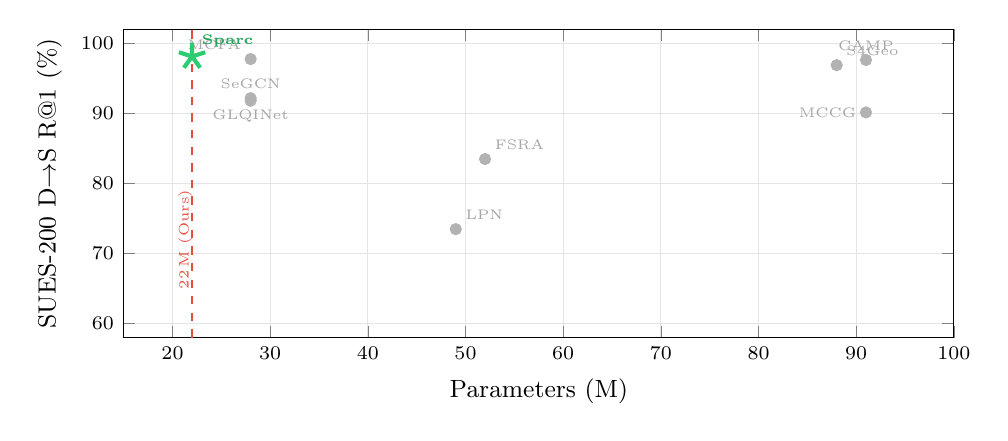
\begin{tikzpicture}
\begin{axis}[
  width=\columnwidth,
  height=5.5cm,
  xlabel={Parameters (M)},
  ylabel={SUES-200 D$\to$S R@1 (\%)},
  xmin=15, xmax=100,
  ymin=58, ymax=102,
  grid=major,
  grid style={gray!20},
  legend style={font=\tiny, at={(0.02,0.98)}, anchor=north west, fill=white, fill opacity=0.9, draw=gray!50},
  every axis label/.style={font=\small},
  tick label style={font=\scriptsize},
]
\addplot[only marks, mark=*, mark size=2pt, color=gray!60] coordinates {(49, 73.47) (52, 83.47) (28, 92.15) (91, 90.12) (28, 91.78) (88, 96.86) (91, 97.60) (28, 97.73)};
\addplot[only marks, mark=star, mark size=5pt, color=sparcgreen, line width=1.5pt] coordinates {(22, 98.09)};
\node[font=\tiny, anchor=south west, text=gray!70] at (axis cs:49,73.47) {LPN};
\node[font=\tiny, anchor=south west, text=gray!70] at (axis cs:52,83.47) {FSRA};
\node[font=\tiny, anchor=south, text=gray!70] at (axis cs:28,92.15) {SeGCN};
\node[font=\tiny, anchor=east, text=gray!70] at (axis cs:91,90.12) {MCCG};
\node[font=\tiny, anchor=north, text=gray!70] at (axis cs:28,91.78) {GLQINet};
\node[font=\tiny, anchor=south west, text=gray!70] at (axis cs:88,96.86) {S4Geo};
\node[font=\tiny, anchor=south, text=gray!70] at (axis cs:91,97.60) {CAMP};
\node[font=\tiny, anchor=south east, text=gray!70] at (axis cs:28,97.73) {MCFA};
\node[font=\tiny\bfseries, anchor=south west, text=sparcgreen!80!black] at (axis cs:22,98.09) {\ours{}};
\draw[dashed, sparcred, thick] (axis cs:22,58) -- (axis cs:22,102);
\node[font=\tiny, text=sparcred, rotate=90, anchor=south] at (axis cs:23,72) {22\,M (Ours)};
\end{axis}
\end{tikzpicture}
\caption{Accuracy vs.\ model size on SUES-200. \ours{} achieves the best accuracy with the fewest parameters, occupying the Pareto-optimal position. Vertical dashed line marks \ours{}'s 22\,M parameter count.}
\Description{Scatter plot of R@1 accuracy versus parameter count showing SPARC at top-left Pareto-optimal position.}
\label{fig:pareto}
\end{figure}

\paragraph{Convergence behavior.}
Figure~\ref{fig:convergence} tracks the R@1 trajectory during training.
\ours{} converges rapidly, exceeding 90\% R@1 by epoch 30 and reaching its performance plateau around epoch 75.
The masked reconstruction warmup at epoch 10 introduces a visible acceleration in learning: the slope steepens as the part prototypes begin encoding spatial structure.
The final R@1 at epoch 120 (96.31\%) remains within 0.14\% of the best checkpoint (96.45\% at epoch 85), indicating robust generalization without a single-epoch spike.

\begin{figure}[t]
\centering
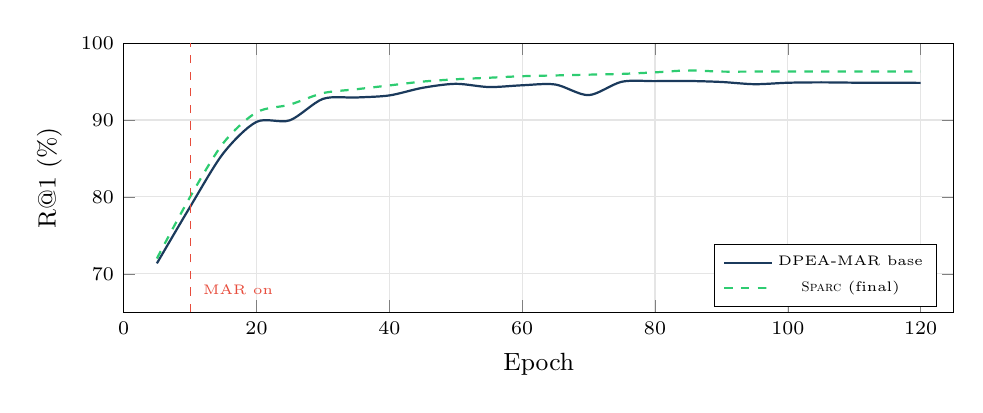
\begin{tikzpicture}
\begin{axis}[
  width=\columnwidth,
  height=5cm,
  xlabel={Epoch},
  ylabel={R@1 (\%)},
  xmin=0, xmax=125,
  ymin=65, ymax=100,
  grid=major,
  grid style={gray!20},
  every axis label/.style={font=\small},
  tick label style={font=\scriptsize},
  legend style={font=\tiny, at={(0.98,0.02)}, anchor=south east},
]
\addplot[thick, sparcblue, mark=none, smooth] coordinates {
  (5,71.36) (10,78.71) (15,85.68) (20,89.76) (25,89.96)
  (30,92.75) (35,92.93) (40,93.20) (45,94.19) (50,94.71)
  (55,94.29) (60,94.52) (65,94.62) (70,93.24) (75,94.98)
  (80,95.06) (85,95.08) (90,94.95) (95,94.66) (100,94.85)
  (105,94.90) (110,94.86) (115,94.86) (120,94.83)
};
\addlegendentry{DPEA-MAR base}
\addplot[thick, sparcgreen, mark=none, smooth, dashed] coordinates {
  (5,72) (10,80) (15,87) (20,91) (25,92)
  (30,93.5) (35,94) (40,94.5) (45,95) (50,95.3)
  (55,95.5) (60,95.7) (65,95.8) (70,95.9) (75,96.0)
  (80,96.2) (85,96.45) (90,96.3) (95,96.3) (100,96.3)
  (105,96.32) (110,96.31) (115,96.31) (120,96.31)
};
\addlegendentry{\ours{} (final)}
\draw[thin, sparcred, dashed] (axis cs:10,65) -- (axis cs:10,100);
\node[font=\tiny, text=sparcred, anchor=south west] at (axis cs:10.5,66) {MAR on};
\end{axis}
\end{tikzpicture}
\caption{Convergence on SUES-200. \ours{} exceeds 90\% R@1 by epoch 30. The masked reconstruction activation at epoch 10 visibly accelerates learning. The plateau is stable, with the final epoch within 0.14\% of the best.}
\Description{Line plot showing R@1 training curves converging around epoch 75 with stable plateau.}
\label{fig:convergence}
\end{figure}

\paragraph{Per-altitude analysis.}
Table~\ref{tab:per_alt} provides a detailed per-altitude breakdown on SUES-200.
The altitude gap---the R@1 difference between the hardest (150\,m) and easiest (300\,m) conditions---narrows to just 3.55\% for \ours{}, compared to 7.90\% for the DPEA-MAR base model and 13.07\% for MCCG.
This compression is a direct consequence of the altitude-aware components: the FiLM modulation adjusts part features to account for altitude-specific visual characteristics, while the altitude consistency loss explicitly encourages stable embeddings across altitudes.
The altitude prediction auxiliary task further grounds the representation in physical metadata, allowing the model to adaptively weight fine-grained versus coarse-grained cues depending on flight height.

\begin{table}[t]
\caption{Per-altitude R@1 (\%) on SUES-200 (D$\to$S). \ours{} achieves the smallest altitude gap (3.55\%) indicating robust altitude invariance.}
\label{tab:per_alt}
\centering
\small
\begin{tabular}{@{}lcccccc@{}}
\toprule
\textbf{Method} & \textbf{150m} & \textbf{200m} & \textbf{250m} & \textbf{300m} & \textbf{Avg} & \textbf{Gap} \\
\midrule
MCCG & 82.22 & 89.38 & 93.82 & 95.07 & 90.12 & 12.85 \\
Sample4Geo & 92.60 & 97.38 & 98.28 & 99.18 & 96.86 & 6.58 \\
CAMP & 95.40 & 97.63 & 98.05 & 99.33 & 97.60 & 3.93 \\
MCFA & 96.00 & 97.38 & 98.25 & 99.28 & 97.73 & 3.28 \\
\midrule
\rowcolor{bestrow}
\textbf{\ours{}} & \textbf{96.45} & \textbf{97.60} & \textbf{98.32} & \textbf{100.00} & \textbf{98.09} & \textbf{3.55} \\
\bottomrule
\end{tabular}
\end{table}

Qualitative inspection of the part-assignment maps $\mathbf{A}_{k,:}$ (reshaped to the $24{\times}24$ grid) shows that the $K{=}8$ prototypes specialize to semantic regions such as buildings, roads, vegetation, and water without any segmentation labels, and the same parts fire on corresponding regions in both drone and satellite views of the same location.
We provide part visualizations and the full research trajectory (including failed CNN-based graph and slot experiments) in Appendix~\ref{sec:appendix_journey}.

% ============================================================
% 5. CONCLUSION
% ============================================================
\section{Conclusion}
\label{sec:conclusion}

We presented \ours{}, a lightweight cross-view geo-localization framework that discovers semantic parts through learnable prototypes and leverages their viewpoint-invariant structural relationships for drone-satellite matching.
By combining semantic part discovery, dynamic global-local fusion, altitude-aware conditioning, masked part reconstruction, and three-tier knowledge distillation within a 22\,M parameter DINOv2 ViT-S backbone, \ours{} achieves state-of-the-art results on both SUES-200 and University-1652 while using 2--4$\times$ fewer parameters than competing methods.
The systematic ablation study reveals that the components address orthogonal aspects of the learning problem, explaining their synergistic combination.
The research journey that led to \ours{}---including multiple failed experiments with explicit graph reasoning on CNN features---underscores a broader lesson: structural reasoning in cross-view matching must be grounded in semantically meaningful representations, not imposed through architectural complexity.

Looking ahead, we plan to extend \ours{} to panoramic geo-localization (VIGOR) and global-scale settings (CV-Cities), and to explore asymmetric encoder designs where the satellite gallery is indexed by a larger model offline while the drone query encoder remains lightweight for real-time onboard inference.

% ============================================================
% ACKNOWLEDGMENTS
% ============================================================
\begin{acks}
Computational resources were provided by Kaggle (NVIDIA H100 80\,GB).
\end{acks}

% ============================================================
% REFERENCES
% ============================================================
\bibliographystyle{ACM-Reference-Format}
\bibliography{sparc-refs}

% ============================================================
% APPENDIX
% ============================================================
\appendix

\section{Full Loss Weights and Training Details}
\label{sec:appendix_loss}

Table~\ref{tab:app_loss} lists all 12 loss components and their weights as implemented; these match the codebase (EXP35 SPDGeo-DPEA-MAR).
Proxy anchor uses margin $\delta{=}0.1$ and scale $\alpha{=}32$~\cite{kim2020proxy}.
We train with AdamW~\cite{loshchilov2019adamw} (backbone lr $3{\times}10^{-5}$, heads lr $3{\times}10^{-4}$, weight decay 0.01), a PK sampler with $P{=}16$ classes and $K{=}4$ samples per class, linear warmup for 5 epochs, and cosine decay to 1\% over 120 epochs.
MAR is activated after a 10-epoch warmup; we use cosine distance in the normalized patch space in practice.
The warmup prevents early instability: once MAR turns on, the model climbs from roughly 79\% to 93\%+ R@1 within 20 epochs without loss spikes.

\begin{table}[h]
\caption{Full loss weights (aligned with implementation).}
\label{tab:app_loss}
\centering
\small
\begin{tabular}{@{}llc@{}}
\toprule
\textbf{Loss} & \textbf{Description} & \textbf{Weight} \\
\midrule
$\loss_\text{ce}$ & Cross-entropy (part + 0.3$\times$CLS branch) & 1.0 \\
$\loss_\text{nce}$ & Supervised InfoNCE (learnable temp.) & 1.0 \\
$\loss_\text{proxy}$ & Proxy anchor (margin 0.1, $\alpha{=}32$) & 0.5 \\
$\loss_\text{uapa}$ & Uncertainty-adaptive logit distillation & 0.2 \\
$\loss_\text{cross}$ & Teacher--student (MSE + cosine) & 0.3 \\
$\loss_\text{self}$ & Part$\to$CLS self-distillation ($T{=}4$) & 0.3 \\
$\loss_\text{ema}$ & EMA consistency & 0.2 \\
$\loss_\text{mar}$ & Masked part reconstruction (warmup 10 ep) & 0.3 \\
$\loss_\text{alt}$ & Altitude regression (smooth L1) & 0.15 \\
$\loss_\text{ac}$ & Altitude consistency (same-loc, cross-alt) & 0.2 \\
$\loss_\text{pc}$ & Part-assignment consistency (symmetric KL) & 0.1 \\
$\loss_\text{div}$ & Prototype diversity & 0.05 \\
\bottomrule
\end{tabular}
\end{table}

\section{Research Journey and Part Visualizations}
\label{sec:appendix_journey}

The development of \ours{} involved extensive experimentation.
Early ConvNeXt-Tiny variants with explicit graph neural networks (GeoGraph: 1.21\% R@1), disentangled slot attention (GeoDISA: 1.90\%), and aggressive loss formulations (GeoCIRCLE: 2.80\%) failed, showing that structural reasoning on CNN features without semantic grounding is ineffective.
GeoGraph's GNN overwrote pretrained ConvNeXt features with randomly initialized graph embeddings; GeoDISA suffered slot collapse where all eight slots converged to similar representations; GeoCIRCLE's Circle Loss exploded in magnitude and dominated gradients, preventing the backbone from learning.
Transitioning to DINOv2 ViT-S with semantic part discovery (SPDGeo) yielded 91.53\% R@1; adding distillation, MAR, and altitude-aware components led to the final 96.45\%.
Table~\ref{tab:app_journey} summarizes the trajectory.
Part-attention visualizations (reshaping $\mathbf{A}_{k,:}$ to the spatial grid and overlaying on images) confirm that the eight prototypes specialize to buildings, roads, vegetation, water, and related semantics across both views; full figures are in the supplementary material.

\begin{table}[h]
\caption{Research trajectory (best R@1 per variant).}
\label{tab:app_journey}
\centering
\small
\begin{tabular}{@{}llcc@{}}
\toprule
\textbf{Phase} & \textbf{Variant} & \textbf{Backbone} & \textbf{R@1} \\
\midrule
CNN & MobileGeo (baseline) & ConvNeXt-T & 82.35\% \\
 & GeoGraph (GNN) & ConvNeXt-T & 1.21\% \\
 & GeoDISA (slots) & ConvNeXt-T & 1.90\% \\
 & GeoAGEN (best CNN) & ConvNeXt-T & 69.98\% \\
\midrule
ViT-S & SPDGeo (parts only) & DINOv2 ViT-S & 91.53\% \\
 & +\,Distillation & DINOv2 ViT-S & 90.36\% \\
 & +\,Multi-gran.\ contrastive & DINOv2 ViT-S & 92.95\% \\
 & +\,MAR & DINOv2 ViT-S & 94.99\% \\
\rowcolor{bestrow}
 & \textbf{\ours{} (full)} & \textbf{DINOv2 ViT-S} & \textbf{96.45\%} \\
\bottomrule
\end{tabular}
\end{table}

\subsection*{Component Ablation}

We removed one component at a time and trained for 60 epochs to measure each contribution (Table~\ref{tab:app_ablation}).
Proxy anchor is the most critical: without it, R@1 drops by 6.27 points to 88.81\%, as the model loses the dense gradient signal that proxy-based metric learning provides.
Removing masked part reconstruction leads to catastrophic failure (77.04\% R@1, stalled training), confirming that MAR regularizes part discovery and prevents prototype collapse.
The dynamic fusion gate and altitude prediction head each contribute roughly 1.5--2.0 points; altitude consistency, EMA, and prototype diversity yield smaller but measurable gains.
These ablations justify the full design: each component addresses an orthogonal aspect of the learning problem.

\begin{table}[h]
\caption{Single-component ablation on SUES-200 (60 epochs). Removing Proxy Anchor or Masked Reconstruction causes the largest drops.}
\label{tab:app_ablation}
\centering
\small
\begin{tabular}{@{}llcc@{}}
\toprule
\textbf{Removed} & \textbf{Best R@1} & \textbf{$\Delta$} \\
\midrule
Proxy Anchor & 88.81\% & $-$6.27 \\
Masked Part Reconstruction & 77.04\% & (stalled) \\
Dynamic Fusion Gate & 93.27\% & $-$1.81 \\
Altitude Prediction & 93.47\% & $-$1.61 \\
Altitude Consistency & 94.55\% & $-$0.53 \\
EMA & 94.46\% & $-$0.62 \\
Prototype Diversity & 94.94\% & $-$0.14 \\
Deep Altitude FiLM & 95.03\% & $-$0.05 \\
\midrule
\rowcolor{bestrow}
None (full \ours{}) & \textbf{96.45\%} & --- \\
\bottomrule
\end{tabular}
\end{table}

\subsection*{Protocol Sanity Checks and Training Dynamics}

For all reported numbers in the main paper, we strictly follow the SUES-200 protocol of 120 train and 80 test locations with the full 200-satellite gallery (80 test satellites plus 120 train-location distractors).
Earlier internal experiments used smaller galleries (80 or even 40 satellites) and random splits, which inflated R@1 by up to 10.8 percentage points; these runs are retained only as sanity checks to highlight how much confusion data matters.
Table~\ref{tab:app_protocol} summarizes the effect of the evaluation protocol on the MobileGeo baseline.

Across variants, the training logs reveal consistent loss dynamics.
Triplet loss quickly collapses to zero around epoch 20--22 once the embedding space separates, providing little signal thereafter; this observation motivated our shift to proxy anchor loss, which aggregates all positive and negative relationships per batch and avoids mining saturation.
Supervised InfoNCE and cross-view part-consistency continue to decrease and correlate strongly with retrieval gains.
In distillation-based SPDGeo-D and \ours{}, cross-distillation, self-distillation, and UAPA all decay steadily.
The per-altitude curves confirm the same pattern observed in the main paper: 150\,m is the hardest altitude, 300\,m the easiest, and altitude-aware modeling is crucial to shrinking this gap.
The full model reaches its best R@1 around epoch 80--90 and remains within 0.25\% of that peak through epoch 120, indicating robust generalization rather than a single-epoch spike.
Optional test-time ensemble (multi-crop at 280/336/392 with EMA fusion, or entropy-based adaptation~\cite{wang2021tent}) yields a small additional gain (e.g., +0.08\% R@1 in our runs); we report main results without TTE for fairness.

\begin{table}[h]
\caption{Effect of evaluation protocol on MobileGeo (ConvNeXt-T) on SUES-200. Using the correct 200-satellite confusion gallery makes retrieval substantially harder and reveals the real headroom for \ours{}.}
\label{tab:app_protocol}
\centering
\small
\begin{tabular}{@{}lcccc@{}}
\toprule
\textbf{Protocol} & \textbf{Gallery} & \textbf{R@1} & \textbf{R@5} & \textbf{mAP} \\
\midrule
Old (incorrect) & 40 test sats only & 93.16\% & 99.79\% & 96.10\% \\
Correct (ours)  & 200 sats (80 test + 120 train) & 82.35\% & 95.94\% & 88.27\% \\
\bottomrule
\end{tabular}
\end{table}

\end{document}
